\documentclass{acm_proc_article-sp}
%\documentclass{sig-alternate}
% Set letter paper size:
%\setlength{\paperheight}{11in}
%\setlength{\paperwidth}{8.5in}
\usepackage{authblk}
%\renewcommand\Authfont{\small}
%\renewcommand\Affilfont{\itshape\footnotesize}
\usepackage{times,amsmath,epsfig}
\usepackage[hyphens]{url}
\usepackage[pagebackref=true]{hyperref}
%\usepackage[hang,raggedright]{subfig}
%\usepackage[font=footnotesize]{subfig}
\usepackage{subfig}
\usepackage{amsmath, graphicx}
%\usepackage{multiFloats}
\usepackage{url}
\usepackage{verbatim}
\usepackage{amssymb,amsmath}
\usepackage{alltt}
%\usepackage{pslatex}
%\usepackage[all]{xy}
\usepackage{color}
\usepackage{listings}

\newcommand\F[1]{\textcolor{red}{F: #1}}
\newcommand\K[1]{\textcolor{red}{K: #1}}
\newcommand\R[1]{\textcolor{red}{R: #1}}

\begin{document}
\title{\textbf{Information Loss During Size Reduction Depending On Structure Scale}}

\author[1]{Laurens Bogaardt}
\author[1]{Romulo Goncalves}
\author[2]{Raul Zurita-Milla}
\author[2,3]{Emma Izquierdo-Verdiguier}

\affil[1]{NLeSC Amsterdam, The Netherlands \vspace{1pt} \{\emph{\{l.bogaardt, r.goncalves\}@esciencecenter.nl}\}}%, o.rubi\}@esciencecenter.nl}\}}
\affil[2]{Faculty of Geo-Information Science and Earth Observation (ITC), University of Twente, the Netherlands \vspace{10pt} \{\{\emph{\{r.zurita-milla,e.izquierdoverdiguier\}@utwente.nl}\}\}}
\affil[3]{Image Processing Laboratory (IPL), Universitat de Valencia, Spain}

\date{} % <--- leave date empty
\maketitle
\thispagestyle{empty} %% <-- you need this for the first page

\begin{abstract}
The analysis of large datasets can be time consuming and costly. Often, techniques exist to arrive at the same output, or at a close approximation, which require far less effort. This article looks at several such techniques and at the inherent scale of the structure within the data. When the values of a dataset vary slowly, e.g. in a spatial field of temperature over a country, there is a high level of autocorrelation and the structure of the field has a large scale. Datasets need not have a high resolution to describe such fields faithfully. Using generated \textit{Gaussian Random Fields} with various levels of spatial autocorrelation, we examine several exact and approximate analysis techniques. Our aim is to outline when certain techniques can be useful and to find a relation between performance and the scale of the structure described by the input datasets.\\ % < Remove \\ later
\end{abstract}

\section{Introduction}
\label{sec:Introduction} %Conclusion: the general rule is to work with square, full rank matrices together with a left- and a right orthonormal rotation matrix.

This article looks at several techniques to analyse large datasets and at the inherent scale of the structure within the data. When a researcher has an idea about the scale of their data and has a target level of accuracy, this article can suggest which technique may be relevant for their analysis. The techniques discussed here are by no means novel~\cite{Golub1970, Bjorck1973, Chan1982}. However, there are domains which are less familiar analysing large datasets, so a review may be beneficial.

\subsection{Matrix Size and Rank Decomposition}
\label{sec:Introduction Matrix Size and Rank Decomposition}

Many datasets can be represented by a matrix of values. Take, for instance, a group of $n$ idividuals who report scores on $m$ different questions. Or take the temperatures at $m$ locations, measured over $n$ time periods. These values can be placed into a matrix with $m$ rows and $n$ columns.

Like a vector, a matrix is a combination of basis vectors, which indicate direction, each with a coefficient, which indicates magnitude. As an extension of the vector, a matrix has two bases, the left- and the right-, or the row- and the column basis. Similarly, these bases can be changed via a rotation. Then, the coefficients will also change, leaving the resulting matrix untouched. A clever basis to rotate into is one where the bases are orthonormal and each subsequent set of left- and right basis vectors explains as much of the remaining variance in the dataset as possible. Such basis vectors are called \textit{Principle Components} or \textit{Empirical Orthogonal Functions} and they may be found via a \textit{Singular Value Decomposition} (\textit{SVD}) of the matrix.

If one can find a rotation in which one of the coefficients becomes zero, the matrix seems to be able to be described by fewer parameters than are available. In a sense, it is underdetermined. It's internal dimension is smaller than what could have been guessed from its $m$ by $n$ size. This is the concept of matrix `rank'. An $m$ by $n$ matrix has rank $r$ if the rows and the columns both span a subspace of dimension $r$. If $r = \text{min}(m, n)$, such a matrix is said to have full rank, the maximum number of linearly independent basis vectors. If $r < \text{min}(m, n)$, it is rank deficient.

A rank decomposition or factorization is the splitting of a matrix into a product where each factor has full rank. For an $m$ by $n$ matrix of rank $r$, with $r \leq n \leq m$, we can decompose it into an $m$ by $r$ matrix and an $r$ by $n$ one. We can choose the first factor of this product to be an orthonormal matrix which induces a rotation, i.e. a change-of-basis. The second factor captures the `action' of the matrix, written in the new bases. It is this second matrix, which is often smaller than the original, which is most relevant for further analyses. An \textit{SVD} is a special type of rank decomposition. It results in a set of orthonormal left basis vectors $U$, a list of coefficients $s$ and a set of right basis vectors $V$. For rank deficient matrices, some the of coefficients, called singular values, will be zero.

As noted by Martinsson, the condition that a dataset has precisely rank $r$ is not realistic in practice because the values originate from devices with finite precision~\cite{Martinsson2016}. Even though some singular values of a dataset are not zero, they may be close enough to zero to be considered \textit{noise}. If we take the inherent imprecise nature of real-world datasets into account, we can approximate a dataset by another matrix of rank $l$, with $l < r$. Following the Eckart-Young-Mirsky theorem, the best possible approximation is one described in the same bases as the original dataset, taking a subset of the $l$ largest singular values and truncating the remainder~\cite{Eckart1936}. Taking a threshold~$\epsilon$, the dataset is said to be approximate rank deficient if some singular values fall below~$\epsilon$. Then, it has an $\epsilon$-rank of $l$ and the norm of the difference with its $l$-rank approximation is at most~$\epsilon$.

So, we can identify three types of matrix `sizes'. The first is the size of the full matrix, $m \times n$. Storing such a matrix requires $m \times n$ units of storage and computing the product with a vector requires $m \times n$ flops~\cite{Martinsson2016}. The second type is the rank decomposed version of the matrix. Storing such a matrix requires $m \times r + r \times n$ units of storage and an equal number of flops for the vector multiplication~\cite{Martinsson2016}. If $r$ is small, this can be a substantial improvement. The final definition of `size' approximates the original dataset with a matrix of rank $l$, resulting in even smaller storage and faster computations, while losing as little information as possible.

\subsection{Spatial Fields}
\label{sec:Introduction Spatial Fields}

In domains such a climate science and phenology, datasets are typically spatial fields, e.g. of temperature. In these fields, values vary slowly and neighbouring points are not entirely independent of one another, neither in space nor in time~\cite{Eshel2011}. Then, there is a high level of autocorrelation and the structure of the field has a large scale. This redundancy means the dataset is rank deficient. In this article, we will examine various fields and exploit rank factorization to analyse the data in an efficient manner. The reported results come from calculations performed in a accompanying \textit{Jupyter Notebook}~\cite{RefNeeded}.

In order to compare analysis techniques and to find the relation between performance and the structure scale, we need to be able to generate fields which resemble fields often encountered in real-world applications. In particular, the field we will concern ourselves with need to have some amount randomness and some level of autocorrelation. Real-valued \textit{Gaussian Random Fields} are particularly useful, as their structure scale can be captured in a single parameter. The power spectrum of such fields follows the power law described by $P(k) = k^{-\alpha}$ where $k$ is the wavenumber and $\alpha$ the parameter which controls the level of autocorrelation. For 2D spatial fields, rotational invariance is assumed, such that $k$ can be substituted by $|\vec{k}|$.

In spatial data analysis, other measures of autocorrelation are often used~\cite{Eshel2011, Storch1999}. These include Moran's I and the $\Gamma$ index~\cite{Moran1950, Hubert1981, PySAL}. Another measure comes from the singular values. These are related to the amount of variance in the original dataset explained by their associated mode. For fields with autocorrelation, the singular values decay quickly. One can try to fit a power law to them and estimate the exponent, which we'll call $\beta$. % The power spectrum gives the data in terms of harmonics. The SVD gives it in terms of empirical observed functions. Therefore, the singular values will always decay more quickly than the amplitude of the wavenumbers, and $\beta$ will be (slightly) larger than $\alpha$.
All the measures give an indication of the level of autocorrelation in the field and the scale of the structure represented in the data. Figure~\ref{fig:plotGammaAndMoransIAndBeta} plots them as a function of $\alpha$ for various generated Gaussian Random Fields.

\begin{figure}[h]
\begin{center}
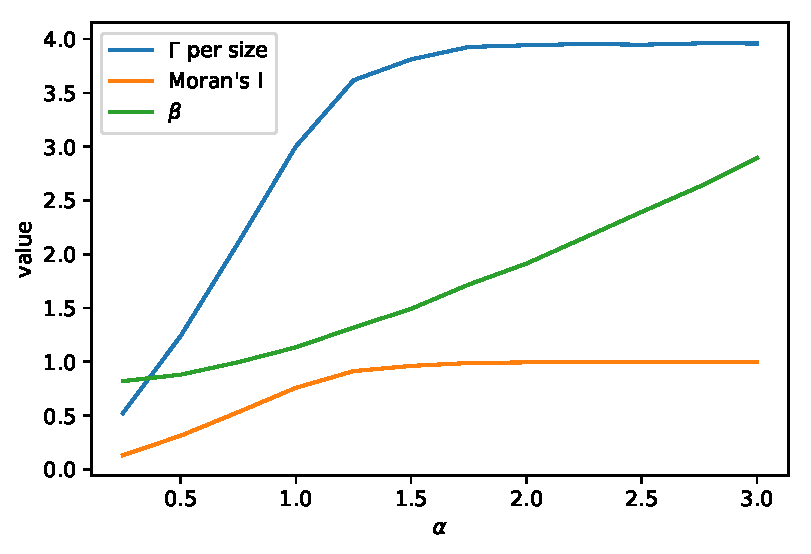
\includegraphics[width=0.8\columnwidth]{Results/plotGammaAndMoransIAndBeta.pdf}
\caption[Various measures of autocorrelation]{Various measures of autocorrelation as a function of $\alpha$}
\label{fig:plotGammaAndMoransIAndBeta}
\end{center}
\end{figure}

\subsection{Spatial-Temporal Fields}
\label{sec:Introduction Spatial-Temporal Fields}

In many real-world applications, the analysis of a field does not only involve a single time snapshot but includes data over multiple weeks, months or years. Then, we are interested in finding patterns which occur frequently. The \textit{maximum covariance analysis} and \textit{canonical correlation analysis} examine the cross-covariance matrix of two datasets and find patterns which occur frequently and simultaneously~\cite{Eshel2011, Storch1999}. Such a pattern, or mode, is a combination of a left- and a right basis vector. One technique to find these modes is to perform an SVD on the product of the standardised datasets. In some domains, the term SVD is used synonymously with MCA. In an MCA, modes are found where the left- and the right-field covary maximally, wereas in an CCA, they correlate maximally~\cite{Bretherton1992}.

Just as there is spatial autocorrelation, there is temporal autocorrelation when the values of the field over the entire time period do not change drastically. In principle, there can be a different level of autocorrelation over time and over space. However, for simplicity, in this article we will use the same $\alpha$ to determine the level of autocorrelation in all dimensions.

\section{Techniques}
\label{Techniques}

This section will discuss four techniques to analyse large datasets efficiently using their singular value decomposition and by exploiting autocorrelation and rank deficiency.

\subsection{Exact Norm of Difference via SVD}
\label{sec:Techniques Exact Norm of Difference via SVD}

One often wants to find the norm of the difference between two fields. This can be done by subtracting one matrix from the other and summing the square of the elements. However, for large matrices, this may be inefficient, especially when they are rank deficient and when their SVDs are already known.

Let $|| \cdot ||$ indicate the Frobenius norm, $\left\langle \cdot \right\rangle$ the Frobenius inner product and the $\circ$ operator the Hadamard product, then the norm of the difference between matrices $A$ and $B$ is given by equation~\ref{eq:normDifferenceFromUSVs}.
\begin{equation}
\label{eq:normDifferenceFromUSVs}
\begin{split}
||A-B||^{2} & = ||A||^{2} + ||B||^{2} - 2 \left\langle A, B \right\rangle \\
& = s_{A}^{T} s_{A} +  s_{B}^{T} s_{B} - 2 s_{A}^{T} \left( U_{A}^{T} U_{B} \circ V_{A}^{T} V_{B} \right) s_{B}
\end{split}
\end{equation}

Figure~\ref{fig:normDifferenceFromUSVs} shows that this procedure can determine the norm in an efficient manner, provided the number of singular values is small. The result is mathematically identical to the full calculation, which means that any error will be of the order of machine-precision.

\begin{figure}[h]
\begin{center}
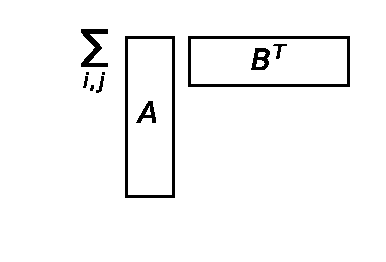
\includegraphics[width=\columnwidth]{Results/normDifferenceFromUSVs.pdf}
\caption[Exact norm difference via SVD]{Exact norm difference via SVD}
\label{fig:normDifferenceFromUSVs}
\end{center}
\end{figure}
%For very large datasets, the SVDs may be obtained using a random algorithm reviewed extensively in an article by Halko et al.~\cite{Halko2011}. The number of singular values will then be truncated to the $l$ largest values, similar to finding an $\epsilon$-rank approximation. In section~\ref{sec:Techniques Approximate SVD via Dimensionality Reduction}, we will also apply this technique to our generated fields. The resulting norm will no longer be exact, but the error can be made arbitrarily small by adjusting $l$ and $\epsilon$.

\subsection{Exact SVD via QR Decomposition}
\label{sec:Techniques Exact SVD via QR Decomposition}
% Using rank(AB) <= min(rank(a), rank(B)).
% Q is an orthogonal matrix (Golub & Van Loan (1996, §5.2) call Q1R1 the thin QR factorization of A; Trefethen and Bau call this the reduced QR factorization.[1]).
% QR decomposition can be achieved via several algorithms, including the Gram–Schmidt process, Householder transformations, or Givens rotations. Each of these has efficiency advantages under different conditions. However, our aim is not to produce the most computationally efficient code, but rather to show that there are multiple routes to arrive at the same output, some of which may be faster than others.

In real-world applications, one often wants to find the relation between two fields. Analyses such as the MCA and CCA discussed in section~\ref{sec:Introduction Spatial-Temporal Fields} rely on performing an SVD of the cross-covariance or cross-correlation matrix of the two fields. In particular, the two input datasets often have the various spatial gridpoints as rows and will have the sample of recorded values over time as columns. Multiplying these gives the cross-correlation matrix. However, for highly rectangular matrices, when there are many spatial gridpoint but few temporal samples, the resulting cross-correlation matrix is inefficiently large and obviously rank deficient. Performing a rank decomposition, such as the \textit{QR Decomposition}, allows one to perform an SVD in an efficient manner~\cite{Chan1982, Tygert2017}. The result is mathematically identical to the full SVD, which means that the difference will be at machine-precision.

\begin{figure}[h]
\begin{center}
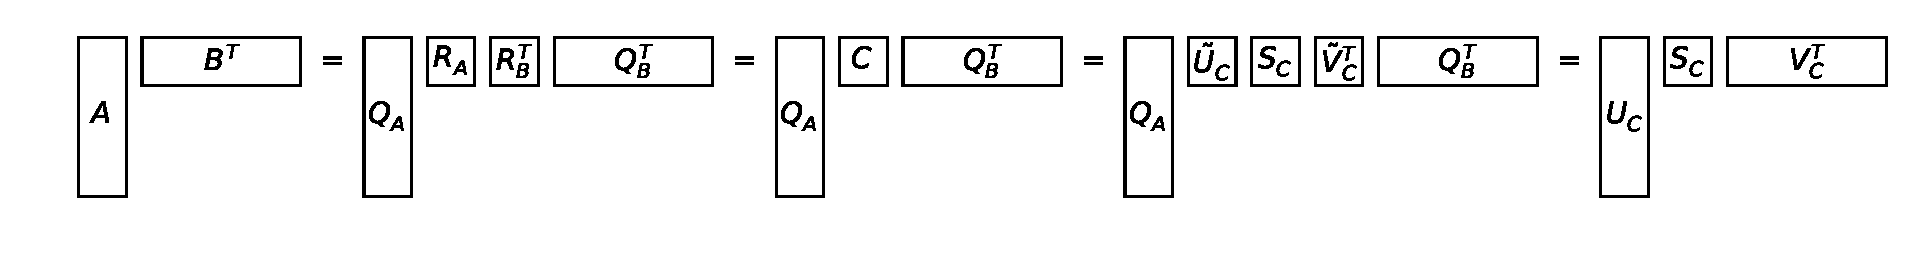
\includegraphics[width=\columnwidth]{Results/qrProductSVD.pdf}
\caption[Exact SVD via QR decomposition]{Exact SVD of a matrix product via QR decomposition}
\label{fig:qrProductSVD}
\end{center}
\end{figure}

\subsection{Approximate SVD via Spatial Coarsening}
\label{sec:Techniques Approximate SVD via Spatial Coarsening}

Although the previous procedure works well for two rectangular matrices, sometimes the input data is large and square. Performing an SVD on such a large dataset will be time consuming and, perhaps, inefficient given the desired level of accuracy. When a spatial field has large scale structure, the values of neighbouring cells do not change drastically. Perhaps neighbouring cells can be aggragated together to produce a smaller dataset which still faithfully describes the original field. In this section, we coarsen various Gaussian Random Fields by averaging patches of neighbouring gridpoints and compare the result with the full calculation.

\begin{figure}[h]
\begin{center}
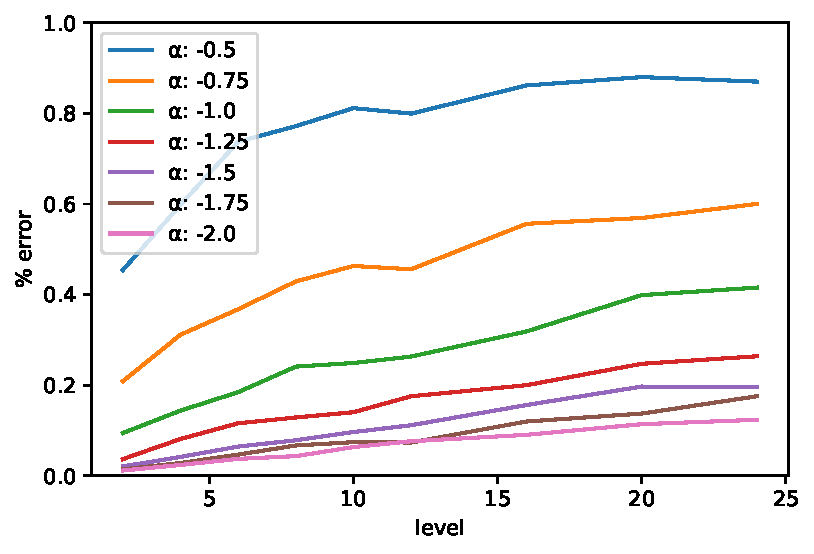
\includegraphics[width=0.8\columnwidth]{Results/plotSingleSpatialFieldViaCoarsening.pdf}
\caption[Error after coarsening a spatial field]{Error after coarsening a spatial field for various $\alpha$'s}
\label{fig:plotSingleSpatialFieldViaCoarsening}
\end{center}
\end{figure}
Figure~\ref{fig:plotSingleSpatialFieldViaCoarsening} shows the percentage error in a coarsening process for matrices of various sizes and $\alpha$'s, and at various levels of coarsening. The error is determined as the norm of the difference between the full calculation and the coarsened version, divided by the norm of the full calculation. The two input matrices used here are similar, as they are generated by the same Gaussian Random Process. Therefore, they will correlate highly and the bases in which they are best described will be similar.

We can also coarsen two different fields before analysing their cross-covariance matrix. Figure~\ref{fig:plotProductSpatialTemporalFieldsViaCoarsening} shows the percentage error for various generated matrices.

\begin{figure}[h]
\begin{center}
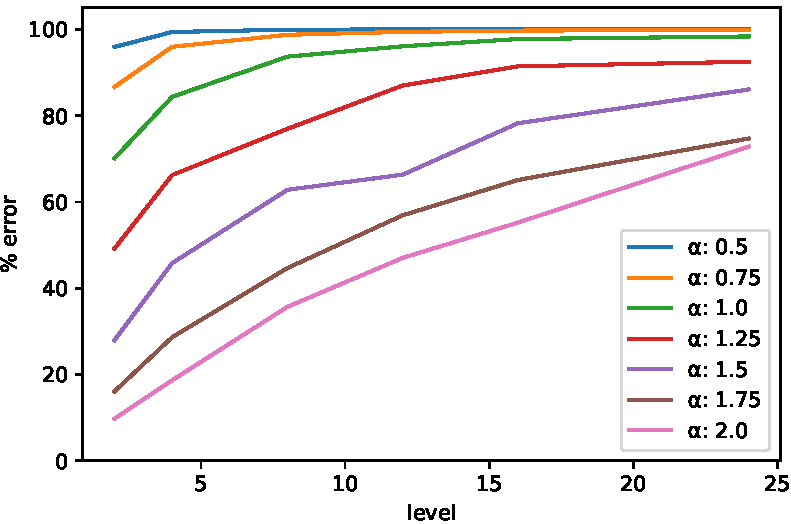
\includegraphics[width=0.8\columnwidth]{Results/plotProductSpatialTemporalFieldsViaCoarsening.pdf}
\caption[Error after coarsening product of fields]{Error after coarsening the product of two fields}
\label{fig:plotProductSpatialTemporalFieldsViaCoarsening}
\end{center}
\end{figure}
Due to the multiplication step in this analysis, the typical error as a result of coarsening is larger than before. As expected, the level of autocorrelation plays an important part, with more negative $\alpha$'s leading to a smaller error. The amount of error during the coarsening process will likely also depend on the similarity between the two datasets. This is one aspect which we do not cover here and leave for further research.

The coarsening process can speed up the calculation of the SVD, but there are additional benefits. When a target level of accuracy is determined, and there is an estimate of the level of autocorrelation of the fields, the data collection process can be optimised. In domains were satellite data is used, datasets are often not very detailed because the imaging resolution is low. Unlike local analyses of developed countries, where high resolution data is becoming more accessible, for continental or global analyses, coarse spatial resolution data may be the only option.

\subsection{Approximate SVD via Dimensionality Reduction}
\label{sec:Techniques Approximate SVD via Dimensionality Reduction}
%Halko:
%-For a matrix that is too large to fit in fast memory, the randomized techniques require only a constant number of passes over the data, as opposed to O(k) passes for classical algorithms. In fact, it is sometimes possible to perform matrix approximation with a single pass over the data
%-Compared with standard deterministic algorithms, the randomized methods are often faster and—perhaps surprisingly—more robust.
%-low-rank matrix approximations
%-The inner dimension k is sometimes called the numerical rank of the matrix. When the numerical rank is much smaller than either dimension m or n, a factorization such as (1.1) allows the matrix to be stored inexpensively and to be multiplied rapidly with vectors or other matrices
%-A basic method in statistics and data mining is to compute the direction s of maximal variance in vector-valued data by performing principal component analysis (PCA) on the data matrix.
%-Another standard technique in data analysis is to perform low-dimensional embedding of data under the assumption that there are fewer degrees of freedom than the ambient dimension would suggest
%-the failure probability decreases superexponentially with the oversampling parameter p
%~\cite{Li2016}
The spatial coarsening process is intuitive and easy to implement. It is not, however, the most efficient way to reduce the size of a dataset. Dimensionality reduction refers to discarding modes which contribute little to the variance in a dataset. An SVD is precisely the procedure used to find modes which explain as much variance as possible. Discarding the smallest singular values/vectors is, therefore, the most efficient form of dimensionality reduction. Performing an SVD on a large dataset, however, is computationally costly. The Randomised Dimensionality Reduction process is far more efficient.

The reduceSizeRandomisedSquare function reduces the input matrix to a smaller square matrix of l by l. It also gives two projection matrices which can bring the rows and columns of this smaller matrix back to the bases of the original input. To make the result more precise, the procedure can be repeated multiple times. The parameter i indicates how many loops are performed.

\begin{figure}[h]
\begin{center}
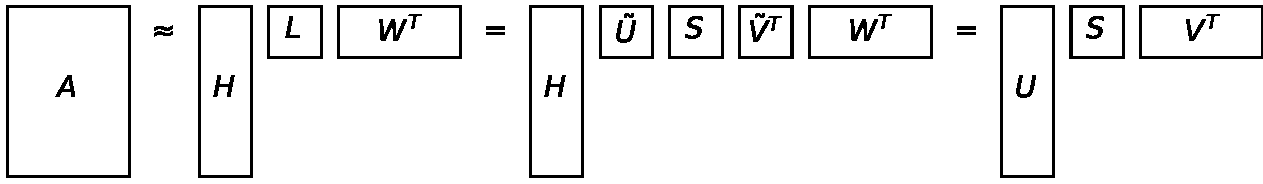
\includegraphics[width=\columnwidth]{Results/reduceSizeRandomisedSquare.pdf}
\caption[Small caption]{Caption}
\label{fig:reduceSizeRandomisedSquare}
\end{center}
\end{figure}
As seen, it is possible for some fields to be represented by matrices of much smaller sizes without losing any substantial amount of information. This is obvious when one realises the singular modes which are removed during the reduction are the smallest ones, described by the tail-end of the power law. In the review article by Halko, Martinsson and Tropp on randomised dimensionality reduction, it is suggested to oversample the reduction. This is because the error introduced in the process is of the same order as the size of the last sampled singular value. If one is interested in the k dominant modes, reducing to a k + l, for some small l, rank approximation will ensure the first k modes are approximated quite well. Indeed, as seen below, the more modes one is interested in, the larger the difference compared with the original matrix.

The Randomised Dimensionality Reduction process can also be applied to the CCA or MCA analysis of two spatial-temporal fields. Similar to the QR Product SVD, it has the advantage that the SVD is applied to a small l x l matrix. The result will be an approximation, but, as we will see, can be close to the real solution.

\begin{figure}[h]
\begin{center}
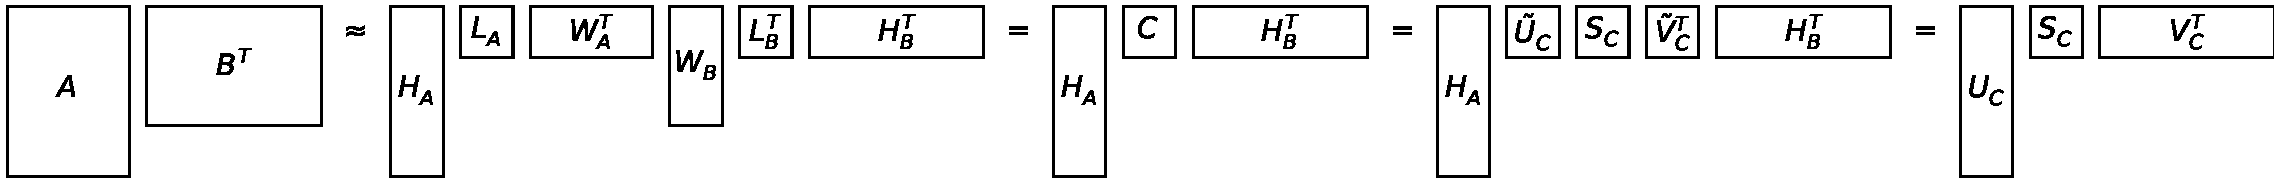
\includegraphics[width=\columnwidth]{Results/randomisedSquareProductSVD.pdf}
\caption[Small caption]{Caption}
\label{fig:randomisedSquareProductSVD}
\end{center}
\end{figure}
To see the effect of dimensionality reduction on such a matrix product, let's generate two Gaussian Random Fields and plot their corss-correlation matrix together with a reduced version. To determine precisely how much information is lost during the reduction, we should look at the variance of the datasets. The norm of the difference between the reduced matrix and the original is the amount of information lost in the reduction process.

\begin{figure}[h]
\begin{center}
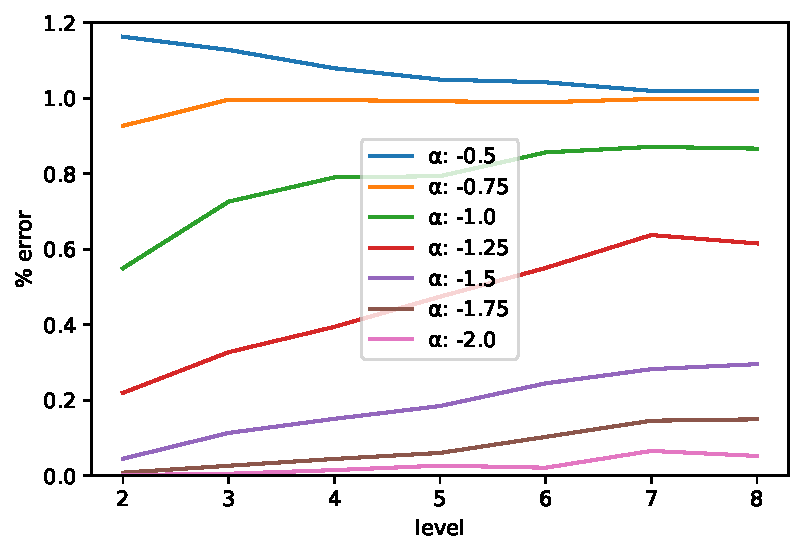
\includegraphics[width=0.8\columnwidth]{Results/plotRandomisedSizeReducedMatrixProduct.pdf}
\caption[Small caption]{Caption}
\label{fig:plotRandomisedSizeReducedMatrixProduct}
\end{center}
\end{figure}
The testRandomisedSizeReducedMatrixProduct function determines the percentage of the information lost in a reduction process for matrices of various sizes and $\alpha$'s, and at various levels of reduction. The two input matrices used here are similar, as they are generated by the same Gaussian Random Process. Therefore, they will correlate highly and the bases in which they are best described will be similar. In principle, any two datasets can be analysed and the amount of information lost during the coarsening process will likely depend on the similarity between the two datasets. This is one aspect which we do not cover here and leave for further research.

Due to the multiplication step in this analysis, the typical error due to reduction is larger than before. There is an affect of temporal size on the information loss. The randomisedSquareProductSVD function is especially useful for square input matrices. To be able to do the comparisons with the full SVD quickly, we use rectangular matrices here. The larger the temporal size, the more square the input matrices. As before, the scale of the structure of the field influences the information loss. The effect in this case can be quite dramatic. Especially for more negative $\alpha$, this procedure performs much better than the coarsening procedure.

Note that, unlike the coarsening procedure, the reduction is not applied on each time-slice of the spatial field, but rather on the spatially-flattened time-series. Therefore, the level of spatial autocorrelation may not be as important as the level of temporal autocorrelation. The proper analysis of this is left for further research.

The reduction of the number of dimensions of each input dataset is actually advised by some researchers, as a method to filter out noise~\cite{Barnett1987}. Especially when the number of temporal samples is small, outliers and random fluctuations could affect the result~\cite{Bretherton1992}. This is because any statistical analysis will choose its regression-coefficients so as to optimize the fit. It may occur that two noise-vectors in the two fields coincidentally covary. In a CCA, where the fields are standardized, this resulting mode may appear important even though it stems from noise. In an MCA, the variance of the noise will be low, so the chance that it will appear as an important mode is less~\cite{Bretherton1992}. One method of finding the right level of filtering is by bootstrapping/cross-validating the results~\cite{Livezey1999}.

%The dimensionality reduction process can speed up the calculation of the SVD, but there are additional benefits. 

\section{Applications}
\label{Applications}

Lorem Ipsum is simply dummy text of the printing and typesetting industry. Lorem Ipsum has been the industry's standard dummy text ever since the 1500s, when an unknown printer took a galley of type and scrambled it to make a type specimen book. It has survived not only five centuries, but also the leap into electronic typesetting, remaining essentially unchanged. It was popularised in the 1960s with the release of Letraset sheets containing Lorem Ipsum passages, and more recently with desktop publishing software like Aldus PageMaker including versions of Lorem Ipsum.

\subsection{Approximate SVD via Spatial Coarsening}
\label{sec:Applications Approximate SVD via Spatial Coarsening}

Lorem Ipsum is simply dummy text of the printing and typesetting industry. Lorem Ipsum has been the industry's standard dummy text ever since the 1500s, when an unknown printer took a galley of type and scrambled it to make a type specimen book. It has survived not only five centuries, but also the leap into electronic typesetting, remaining essentially unchanged. It was popularised in the 1960s with the release of Letraset sheets containing Lorem Ipsum passages, and more recently with desktop publishing software like Aldus PageMaker including versions of Lorem Ipsum.

\subsection{Approximate SVD via Dimensionality Reduction}
\label{sec:Applications Approximate SVD via Dimensionality Reduction}

Lorem Ipsum is simply dummy text of the printing and typesetting industry. Lorem Ipsum has been the industry's standard dummy text ever since the 1500s, when an unknown printer took a galley of type and scrambled it to make a type specimen book. It has survived not only five centuries, but also the leap into electronic typesetting, remaining essentially unchanged. It was popularised in the 1960s with the release of Letraset sheets containing Lorem Ipsum passages, and more recently with desktop publishing software like Aldus PageMaker including versions of Lorem Ipsum.

\section{Further Questions}
\label{Further Questions}

It may be interesting to extend this research to fields other than the Gaussian Random Field. This type was chosen because its structure scale can be captured in a single parameter $\alpha$. In many applications, however, the dataset does not resemble such a Gaussian Random Field.

Additionally, it would be an improvement to relax the assumption that the auto-correlation in the time direction is similar to that in the spatial directions. In fact, it may even be more realistic to have different levels of autocorrelation in the $x$ and in the $y$ direction.

Can similar tricks be used to the generalised MCA/CCA analysis, where the input to the SVD in a concatenation of multiple cross-correlation matrices~\cite{Carroll1970, Kettenring1971}?

Can the dimensionality reduction be applied to the spatial part of the spatial-temporal fields, before it is flattened?

Can a randomised algorithm be developed to estimate Moran's I or some other measure of autocorrelation, using a sample of the data?

{
\footnotesize
\bibliographystyle{abbrv}
\bibliography{Bibliography}
}

\end{document}
